%
% Copyright (c) 2024
% Rémy Hubscher - <hubscher DOT remy AT gmail DOT com>
%
% This file may be distributed and/or modified under the terms of 
% the Apache v2 licence
% 

\documentclass{beamer}

\usetheme[shownavigation={false},  % true | false
          utbmlogo={LogoAAA.png},
          logo={logo.png},
          titlepageimage={titleimage.png},
          header=fullnav,          % fullnav | shortnav | utbm
          suiveur={Franck BERTAGNINI},
          dept={Formation FI (A)}
        ]{UTBM}

\usecolortheme{Terra}

\usepackage[francais]{babel}
\usepackage{datetime}  
\usepackage[T1]{fontenc}
\usepackage{lmodern}

\author{Rémy HUBSCHER} 

\AtBeginSection[] {
  \begin{frame}<beamer>{\insertsectionhead}
    \tableofcontents[currentsection,sectionstyle=show/hide,hideothersubsections]
    \end{frame}
}

\begin{document}
  \title[Briefing Long — Conditions VMC]{Les Conditions Météorologique du vol à vue}
  \subtitle{Briefing Long — Conditions VMC}
\date{\today} 

\begin{frame}[plain]
  \titlepage
\end{frame}

\begin{frame}{Objectifs}
  Étudier les conditions VMC minimales réglementaires pour définir la
  météo minimale d'un vol prévu.
\end{frame}

\begin{frame}{Utilité}
  \begin{itemize} 
    \item Savoir dire si le vol prévu est réglementaire au vue des conditions météos ; \pause
    \item Voler en toute sécurité en évitant les traffics, obstacles et les nuages ; \pause
    \item Pouvoir naviguer avec des points de repère au sol (cheminement, points tournant, points d'entrée) ; \pause
    \item Prévenir des situations dangereuses ; \pause
    \item Garantir sa séparation avec les traffics IFR.
  \end{itemize}  
\end{frame}

\begin{frame}{Rapport}
  \textbf{En voiture}
  
  \begin{itemize}
    \item Quelle est la limite de vitesse sur l'autoroute ? \pause sous pluie ? \pause
    \item Quelle est la limite de vitesse lorsque la visibilité est inférieure à 50 m ? \pause
    \item Qu'impose la loi montagne vis à vis de l'équipement des voitures ? \pause
  \end{itemize}

  \vspace*{1em}
  \center{\textbf{En voiture on a une réglementation pour garantir la sécurité en fonction des conditions du jour.}}
  \pause
  
  \vspace*{1em}
  C'est pareil en avion.
\end{frame}

\section{Questions}
\subsection{La visibilité}
\begin{frame}{La visibilité}
  \textbf{Quels phénomènes météos vont avoir un impact sur la visibilité ?}
  
  \begin{itemize}
    \item Brouillard, brûmes, \pause
    \item Précipitations (neige, averses, pluie, orages), \pause
    \item Tempête de sable ou de poussière, \pause
    \item Fumées (feux, centrales nucléaires), \pause
    \item Nuages \pause
  \end{itemize}

\end{frame}

\subsection{Les espaces aériens}
\begin{frame}{Les espaces aériens}
  \textbf{Quelles sont les classes d'espace aérien ?}

  \pause
  \begin{figure}
    \centering
    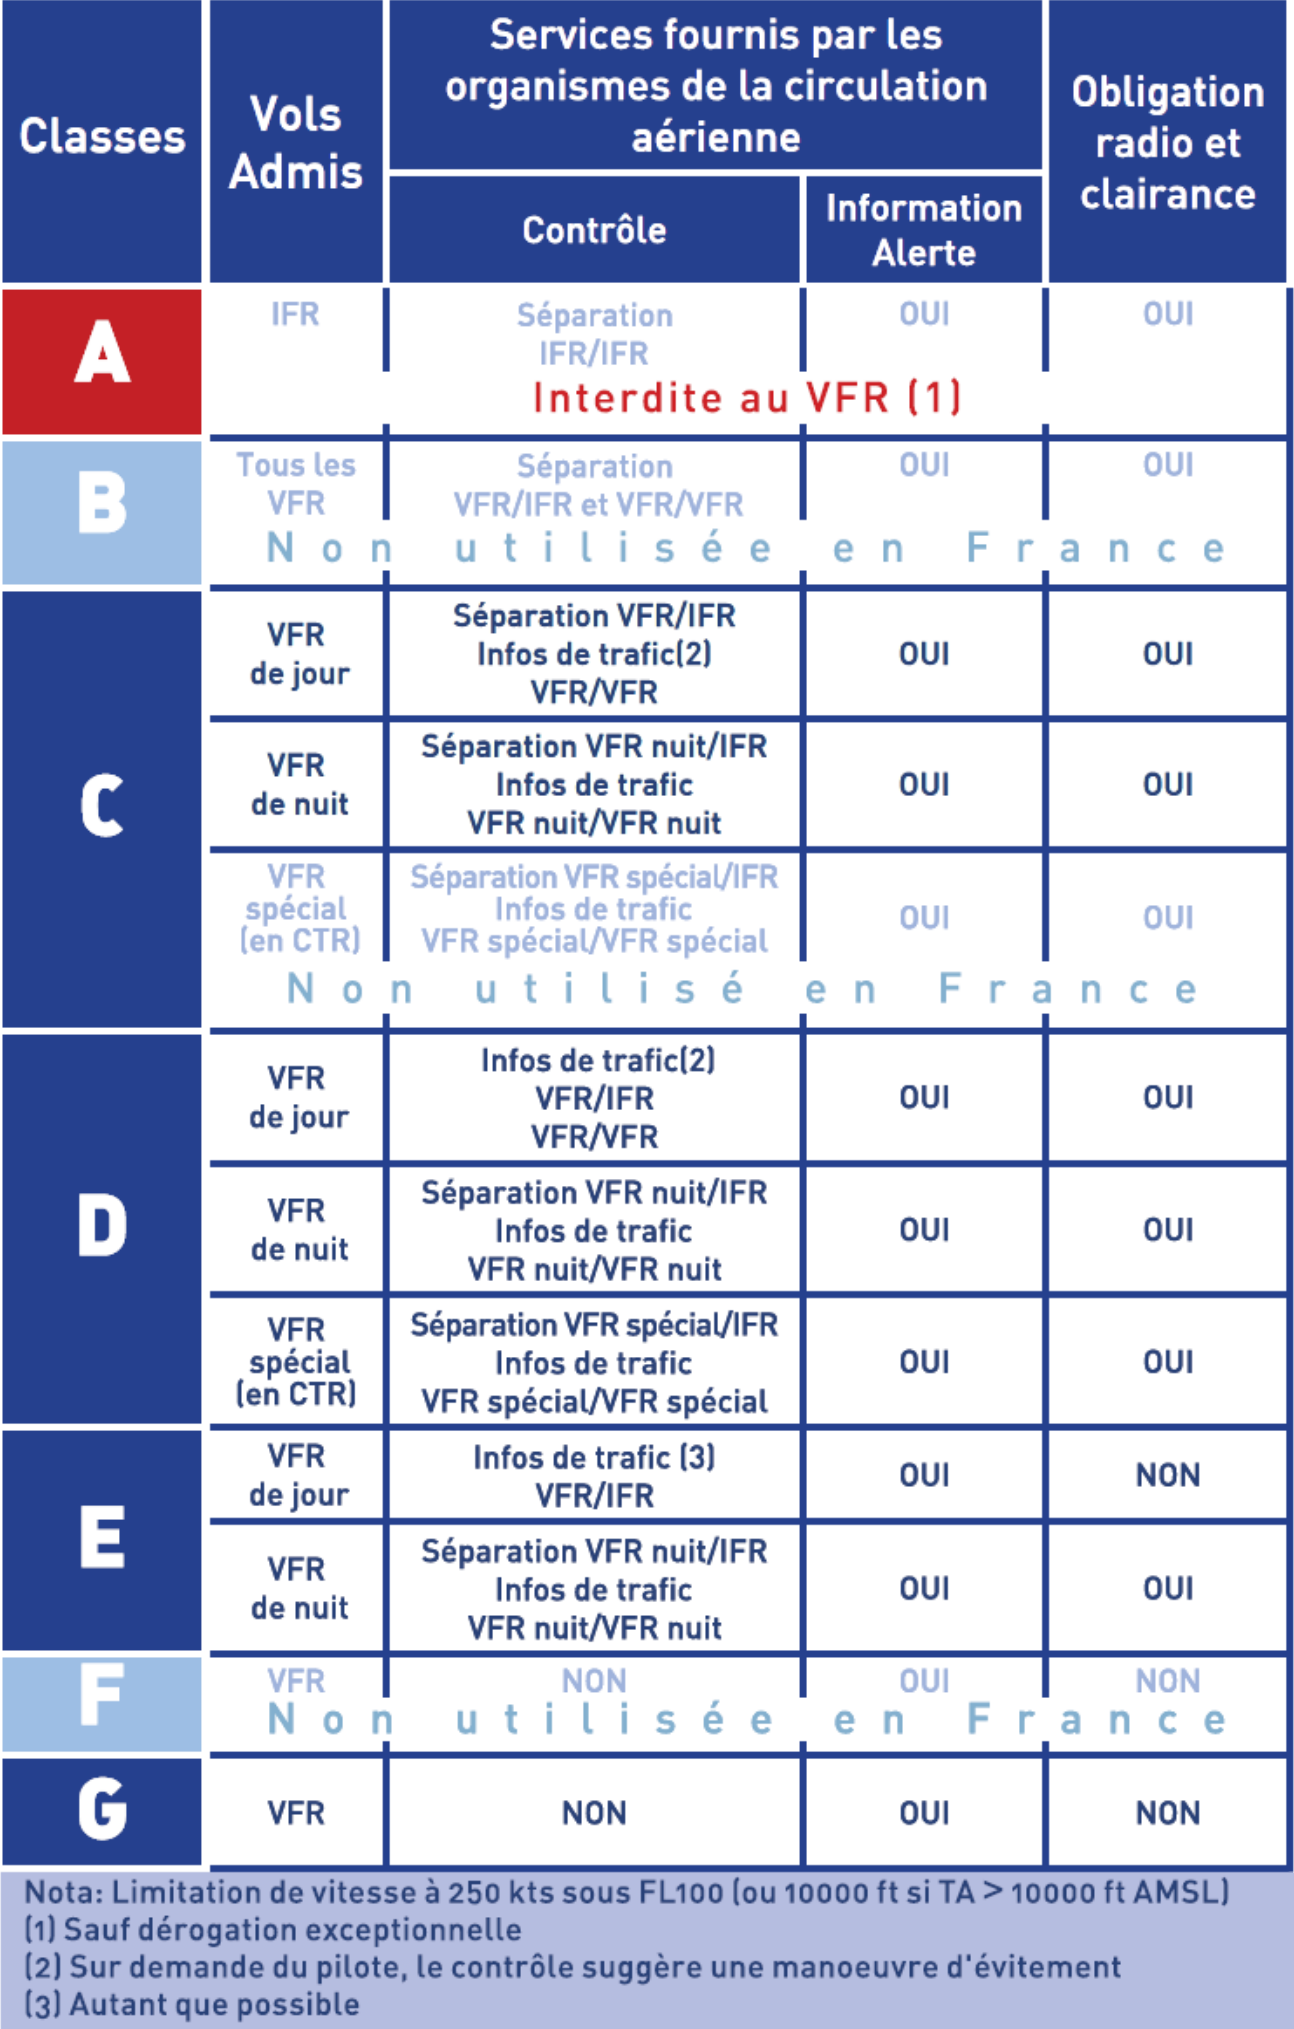
\includegraphics[scale=1.41]{images/espaces-aeriens.png}
  \end{figure}
\end{frame}

\subsection{Le calage altimétrique}
\begin{frame}{Le calage altimétrique}
  \textbf{Qu'est-ce que le QNH et le QFE ?}
  
  \begin{itemize}
    \item QNH : Calage altimétrique donnant l'altitude par rapport au niveau moyen de la mer (AMSL) \pause
    \item QFE : Calage altimétrique donnant la hauteur par rapport au sol (AGL)
  \end{itemize}

\end{frame}

\begin{frame}{Thème}
  \tableofcontents[hideallsubsections]
\end{frame}

\section{Définitions}
\subsection{VMC}
\begin{frame}{VMC — Visual Meteorological Conditions}
  Le terme VMC est définie dans l'Annexe 2 des règles de l'air de l'OACI.
  \vspace*{1em} \pause

  Elle est reprise dans la réglementation européenne le SERA.5 et dans
  sa spécificité française le SERA.FRA.5
  \vspace*{1em} \pause

  Il y est dit que tous les vols VFR doivent respecter des minimas de
  visibilité et d'espacements avec les nuages.
  \vspace*{1em} \pause

  \textbf{Ces minimas dépendent de l'altitude et du type d'espace aérien dans
  lequel l'avion évolue.}

\end{frame}

\subsection{IMC}
\begin{frame}{IMC — Instrument Meteorological Conditions}
  Le terme IMC quant à lui signifie, les conditions météorologiques qui sont inférieures aux conditions VMC.

  \pause
  \begin{figure}
    \centering
    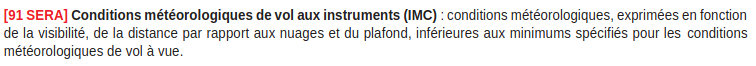
\includegraphics[scale=1.8]{images/sera.imc.png}
  \end{figure}

  \pause

  On constate que contrairement à la croyance populaire, IMC ne veut
  pas dire qu'on est entré dans un nuage, mais que les conditions VMC
  ne sont pas réunies.

  Pour les mêmes conditions on peut donc être en IMC en classe D et en
  VMC en classe G.
\end{frame}

\section{Découpage de l'espace aérien}
\subsection{Découpage vertical}

\begin{frame}{Découpage vertical}
  L'espace aérien se découpe en plusieurs altitudes clés :

  \begin{itemize}
    \item Le vol au dessus du FL195, \pause
    \item Le vol au dessus du FL100, \pause
    \item Le vol en dessous de \textbf{la surface S}.
  \end{itemize}

\end{frame}


\subsection{Découpage spacial}
\begin{frame}{Découpage spacial}
  Les conditions VFR sous le FL100 sont également différentes en
  espace aérien contrôlé et en espace aérien non contrôlé.
\end{frame}

\section{Conditions VMC}
\subsection{Au dessus du FL195}

\begin{frame}{Au dessus du FL195}
  L'Annexe 2 de l'OACI, interdit le VFR au dessus du FL195 sans
  autorisation.
  
  En Europe et en France, l'espace aérien au dessus du FL195 est un
  espace aérien de classe A, il est donc interdit au VFR.

  Il n'y a donc pas de conditions VMC pour cet espace car le vol VFR
  n'y est pas autorisé.
\end{frame}

\subsection{L'espacement avec les nuages}

\begin{frame}{L'espacement avec les nuages}
  Pour éviter une dégradation instantanée de la visibilité, l'OACI
  requiert un espacement avec les nuages :

  \begin{itemize}
    \item 1500m à l'horizontale, \pause
    \item 300m (1000ft) à la verticale.
  \end{itemize}

  Ces règles d'espacement avec les nuages sont valables au dessus de
  la surface S et en espace aérien contrôlé (hors clairance de VFR
  spécial).
  
\end{frame}


\subsection{Au dessus du FL100}

\begin{frame}{Au dessus du FL100}
  Au dessus du niveau 100, la vitesse n'est pas limitée.

  Les conditions VMC nécessitent une visibilité de 8 kms.
\end{frame}

\subsection{Au dessous du FL100}

\begin{frame}{Au dessous du FL100}
  Au dessous du niveau 100, la vitesse est limitée à 250kt.

  Les conditions VMC nécessitent une visibilité de 5 kms.
\end{frame}


\subsection{Sous la surface S}

\begin{frame}{La surface S}
  La surface S correspond à l'espace entre :

  \begin{itemize}
    \item Le sol et la plus haute valeur entre : \pause
    \item 1000 ft AGL (QFE), et 3000 ft AMSL (QNH). \pause
  \end{itemize}

  \pause
  \begin{figure}
    \centering
    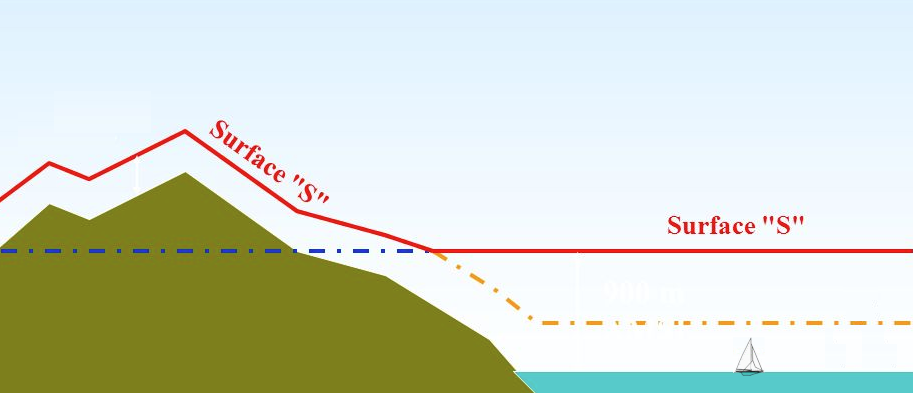
\includegraphics[scale=1.2]{images/surface-s.png}
  \end{figure}
  
\end{frame}

\begin{frame}{Conditions en espace aérien non contrôlé sous la surface S}
  En espace aérien non contrôlé, sous la surface S, les conditions VMC sont :

  \pause
  
  \begin{itemize}
    \item Hors des nuages en vue du sol, \pause
    \item 1500m de visibilité en dessous ($\leq$) de 140kt, \pause
    \item 5000m de visibilité au dessus de 140kt.
  \end{itemize}

\end{frame}

\begin{frame}{Conditions en espace aérien non contrôlé sous la surface S} 
  Il y a une dérogation pour les avions ne pouvant ralentir à 140 kt :

  \vspace*{1em} \pause

  30 secondes de vol de visibilité à plus de 15 kms d'un aérodrome ou
  au départ / arrivé sur ce dernier.

  \vspace*{1em} \pause
  En divisant la vitesse en nœuds par 2 on obtiens les m/s.

  \vspace*{1em} \pause
  $140 kt \Rightarrow 70m/s$ soit 2100m de visi en 30 secondes.

  \vspace*{1em} \pause
  \center{\textbf{Pour avoir 30 secondes avec 1500m de visi, \\il conviendrait de voler à 100kt.}}
  
\end{frame}

\subsection{Le VFR spécial}

\begin{frame}{Le VFR spécial}

  Le SERA.5010 définit des règles de VFR spécial en zone de contrôle.
  \pause

  Le VFR spécial nécessite une clairance du contrôle et doit être
  demandé par le pilote.

\end{frame}
  
\begin{frame}{Le VFR spécial — côté pilote}

  \begin{itemize}
    \item Le VFR spécial peut-être effectué de jour uniquement, \pause
    \item Le pilote doit évoluer hors des nuages, en vue du sol, \pause
    \item 1500m de visibilité, \pause
    \item Une vitesse de 140kt ou moins pour permettre l'anti-abordage.
  \end{itemize}

\end{frame}
  
\begin{frame}{Le VFR spécial — côté organisme de contrôle}
  L'organisme de contrôle ne peut pas délivrer cette clairance si :
  \pause
  
  \begin{itemize}
    \item Le plafond est inférieur à 180m (600ft), \pause
    \item La visibilité au sol est inférieure à 1500m.
  \end{itemize}

\end{frame}

\section{Récapitulatif}

\subsection{Tableau des minimas VMC par classe d'espace aérien}
\begin{frame}{Tableaux récapitulatif des minimas VMC}
  \begin{figure}
    \centering
    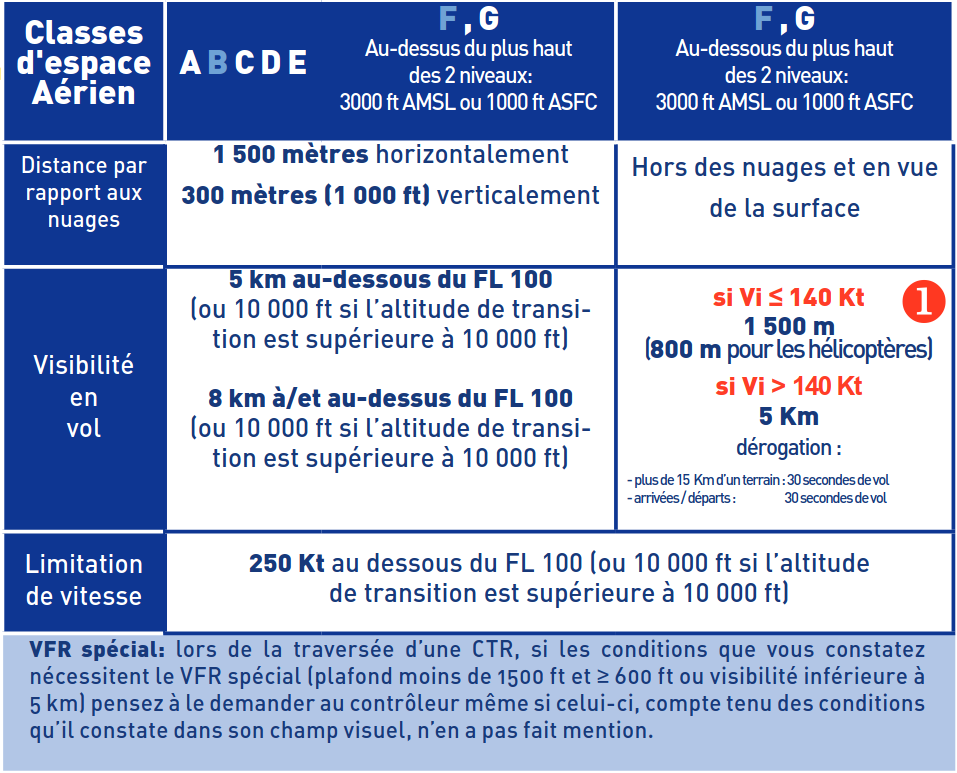
\includegraphics[scale=1]{images/conditions-vmc.png}
  \end{figure}
  
\end{frame}

\subsection{Illustration des VMC selon l'altitude et le type d'espace aérien}
\begin{frame}{Illustration des VMC}
  \begin{figure}
    \centering
    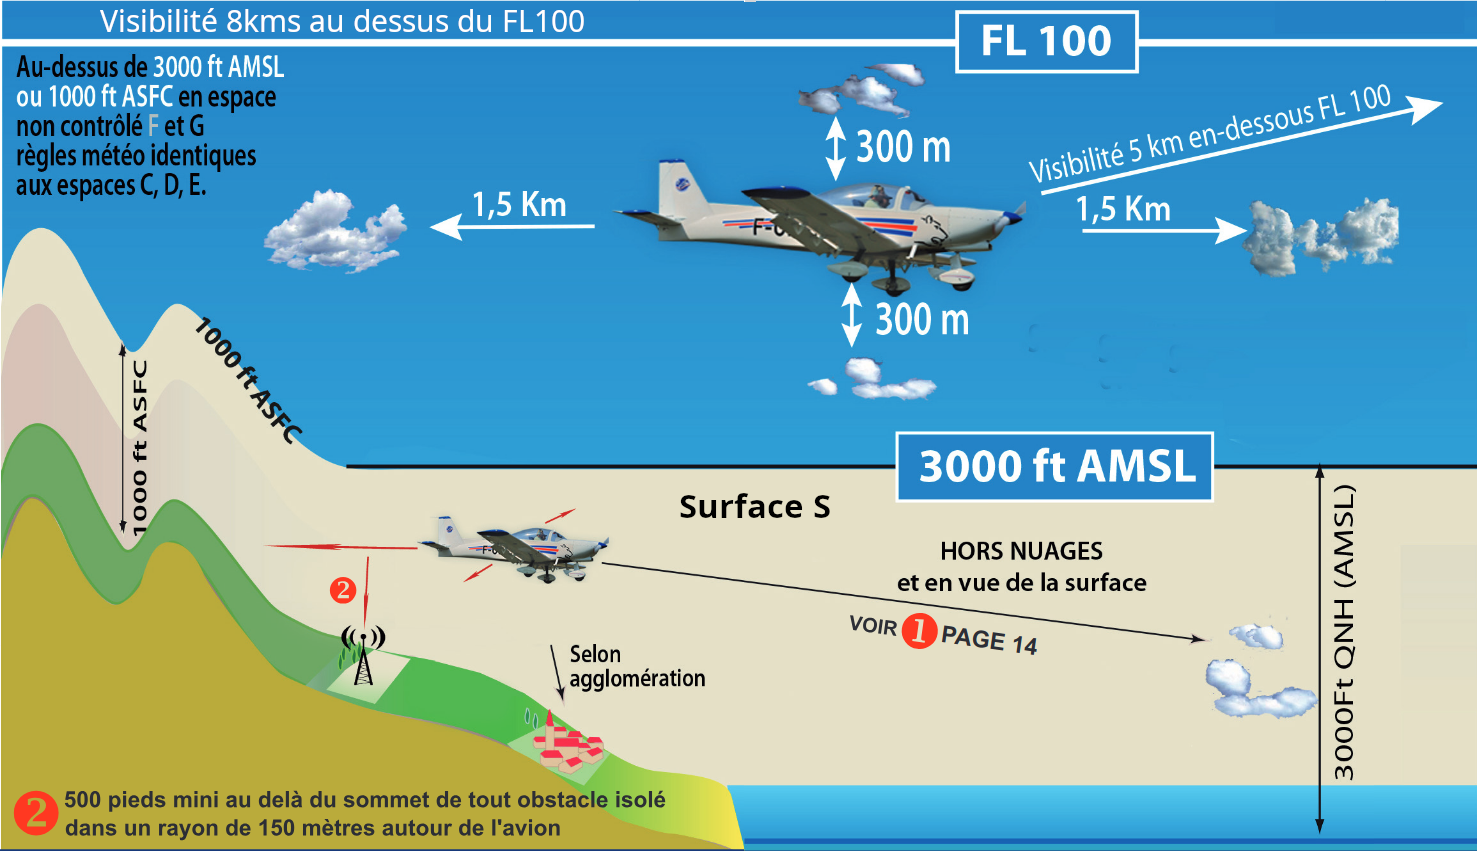
\includegraphics[scale=0.9]{images/conditions-vmc-graphique.png}
  \end{figure}
  
\end{frame}

\subsection{Entrée involontaire en IMC}
\begin{frame}{Entrée involontaire en IMC}
  Une entrée involontaire en IMC nécessite la rédaction d'un CRESAG.
  \vspace*{1em} \pause

  Si tel est le cas, contacter le correspondant sécurité de votre
  aéroclub qui vous aidera à effectuer la démarche CRESAG et le Rex
  FFA.
  \vspace*{1em} \pause

  Il est possible de retrouver toutes ces informations dans
  \textbf{\href{https://www.ffa-aero.fr/siteffaprod_web/fichiers_ffa/Piloter/MemoPiloteVFR.pdf}{le Mémo du Pilote VFR}}.
  
\end{frame}

\section{Exercices}
\subsection{Méthode}

\begin{frame}{Méthode}
  \begin{enumerate}
    \item On trace la route la plus directe, \pause
    \item On regarde l'altitude de survol minimum par rapport à l'obstacle, \pause
    \item On regarde les espaces aériens traversés et on note la visibilité et le plafond (hauteur) de la base des nuages minimal réglementaire, \pause
    \item On ajoute une ligne avec les minimas du pilote et on prends le plus haut des deux entre : réglementaire et minima pilote, \pause
    \item On vérifie si la météo est compatible.
  \end{enumerate}
\end{frame}

\subsection{Définir les minimas VFR nécessaire pour une navigation de Rennes à Dinard}

\begin{frame}{Minimas VFR à Rennes / Dinard}
  Définir les minimas VFR nécessaire pour une navigation de Rennes à Dinard.
\end{frame}

\subsection{Définir les minimas VFR nécessaire pour une navigation de Redon à Plöermel}
\begin{frame}{Minimas VFR de Redon à Ploërmel}
  Définir les minimas VFR nécessaire pour une navigation de Redon à Ploërmel.
\end{frame}

\subsection{La météo est-elle compatible pour un trajet Vichy-Pontarlier ?}
\begin{frame}{Météo compatible pour un trajet Vichy - Pontarlier}
  Avec le dossier météo fournit, est-il possible de rejoindre Pontarlier depuis Vichy ?
\end{frame}



\end{document}
